\documentclass[sigconf]{acmart}

\settopmatter{printacmref=false}
\renewcommand\footnotetextcopyrightpermission[1]{}

%%
%% \BibTeX command to typeset BibTeX logo in the docs
\AtBeginDocument{%
  \providecommand\BibTeX{{%
    Bib\TeX}}}

%% These commands are for a PROCEEDINGS abstract or paper.
\acmConference[APE CS 598]
{APE CS 598}{Spring 2025}{Urbana, IL}

\begin{document}

\title{Java Chess Engine}

\author{Adam McNeil}
\email{adamwm4@illinois.edu}
\affiliation{%
  \country{University of Illinois Urbana-Champaign, Urbana, Illinois, USA}
}

\begin{abstract}
In this paper, we highlight optimizations performed on a Java chess engine.
The goal of these optimizations is to increase the depth that the engine is able to compute efficiently.
Though this does not necessarily make it better at playing chess—since we are computing at a small depth—increasing it will make the chess engine more accurate.
There are also other ways to make the chess engine better, but they are not the focus of this paper.
\end{abstract}

\maketitle
Link to the engine: \url{https://github.com/adamMcneil/chess-engine}

Link to the bot: \url{https://github.com/adamMcneil/cheeky-koala-lichess-bot}

\section{Background}
This project was originally developed by me and a friend in the summer of 2021.
We designed it in an object-oriented way, which was not always the most performant.
This is the original file structure of the project:
\begin{verbatim}
Cheakykoala/
|-- Pieces/
|   |-- Bishop.java
|   |-- Empty.java
|   |-- King.java
|   |-- Knight.java
|   |-- Pawn.java
|   |-- Piece.java
|   |-- Queen.java
|   |-- Rook.java
|-- Board.java
|-- Color.java
|-- Main.java
|-- Move.java
|-- Position.java
|-- PromotionMove.java
\end{verbatim}
\texttt{Piece} is an abstract class that the other pieces inherit from.
\texttt{Color} is an \texttt{Enum} with three values: \texttt{w, b, g}.
These represent white, black, and gray, respectively.
Gray is used for the Empty Piece. Having an Empty Piece to represent a blank square does not seem very efficient, but surprisingly, it does not make a huge impact on performance.
The \texttt{Position} class adds a lot of overhead to the program; all it does is wrap two integers together to represent the position.
It introduces a lot of unnecessary object allocation and function calls.
\texttt{PromotionMove} inherits from the \texttt{Move} class; this is probably not the best way to handle this and should be optimized.

\subsection{Gradle}
In the past, I relied on the IntelliJ IDE for building the project.
Since the project was out of date, it did not work when I revisited it.
So I decided to switch to Gradle for building the project.
This was a good decision because it offers a lot of different actions out of the box, such as running the application, running tests, and generating jar files.

\subsection{IntelliJ}
Since I am a student, I have access to IntelliJ Ultimate. IntelliJ Ultimate offers a lot of features that are very helpful for performance engineering the application.
It has built-in code coverage tools that show what percentage of lines are covered by your tests.
It also provides access to a profiling program that can generate a Flame Graph, Call Tree, Method List, Timeline, CPU Usage, and Events.
It also gives me access to the debugger, which is helpful for debugging.

\subsection{Lichess}
I used an open-source resource \cite{lichess-bot} to connect my chess engine to Lichess.
It uses the Universal Chess Interface (UCI) \cite{uci} to communicate with Lichess.
To use the program, you only need to point it to your chess engine executable and use a YAML config file to configure your chess engine.
It also allows you to use opening books, which are sets of games that the engine will play by default at the beginning of a game \cite{pgn}.

To turn the chess project into an executable, I use Gradle to build the project into a jar file and then use a bash script to execute the file.
This just runs the Java interpreter.
We use the following simple script to run the program:
\begin{verbatim}
#!/bin/bash
java -cp chess-engine-1.0-SNAPSHOT.jar cheekykoala.Main
\end{verbatim}
To communicate with Lichess, your chess engine must respond to very simple inputs described in Table~\ref{tab:api}.

\begin{table*}[h]
    \centering
    \renewcommand{\arraystretch}{1.2}
    \setlength{\tabcolsep}{8pt}
    \begin{tabular}{|c|c|c|}
        \hline
        \textbf{Input} & \textbf{Description} & \textbf{Output} \\
        \hline
        \texttt{uci} & Confirming that the engine is running uci. & \texttt{uciok} \\
        \hline
        \texttt{isready} & Confirming that the engine is ready. & \texttt{readyok} \\
        \hline
        \texttt{position <fen> moves <list of moves>} & Load the board position from the server & \\
        \hline
        \texttt{go wtime <n> btime <n> winc <n> binc <n>} & Output a move that you want to make. & bestmove (e2e4) \\
        \hline
        \texttt{quit} & \texttt{Quit the chess engine} & \\
        \hline
    \end{tabular}
    \caption{A description of the API that the chess engine needs to respond to in order to play on Lichess.}
    \label{tab:api}
\end{table*}

\section{Introduction}
A chess engine consists of a few basic parts.
\begin{enumerate}
    \item \textbf{Move Generation} – Responsible for determining all legal moves from a given board state.
    \item \textbf{Board Evaluation} – Assigns a score or value to a position to help judge its quality.
    \item \textbf{Search Algorithm} – Combines the other components to find the best move in any given state.
\end{enumerate}

\subsection{Move Generation}
This is relatively simple; it just requires you to specify the rules of chess in a programming language. This requires a lot of testing and debugging to cover all of the corner cases (literally the corner cases).
However, the structure of the data you use in this case will affect how efficiently you can produce a list of legal moves.

\subsection{Board Evaluation}
In its simplest form, this is a variable with four possible values.
\begin{itemize}
    \item Black in checkmate
    \item White in checkmate
    \item Stalemate
    \item None
\end{itemize}
However, this is an unrealistic metric because the search space is too massive to find a mate from the starting position, and the bot would see no way to win, so it would play randomly.

The next obvious metric would be material advantage (simply, who has better pieces on the board).
We assign values to each piece and make the black pieces the negative value of the white pieces.
In this way, we can have the player prefer positions where they have better pieces on the board and the other person has fewer pieces on the board. This is a good heuristic for who is winning the game.

However, this does not capture everything that chess players use to determine which side is in a better position.
Players also develop pieces—this usually means moving pieces toward the center of the board or having a good pawn structure.
To capture this, we can use a table of values that offers a small benefit to pieces in each of those positions.
Each piece has a separate table of values that is used to determine the benefit of each piece in a specific location on the board.
Intuitively, this is because it is better to have your king in the back protected, and for pawns, it is good to have them on the second-to-last row so that they are close to promoting.

\subsection{Move Search}
Since chess is a two-player game, it uses a minimax algorithm to find the best move.
There are better explanations of this algorithm online, but at a basic level, the computer takes turns maximizing and minimizing the branching board state. This simulates both players playing optimally and allows the computer to compute the most optimal solution.

Now that we have a move generator and a way to compare boards, we can use standard graph algorithms to search for the best move.
The most basic search would be a depth search.
However, this is not optimal in chess because the player needs to move in real time.
It is hard to know how long the depth search will take.
Because of this, it is hard to determine what depth the bot should search for.
Furthermore, the search needs to complete before it finds a move.

The algorithm that is best for looking for moves in chess is iterative deepening.
It works by doing consecutive executions of a depth search.
This allows the bot to return the best move it has found after it has reached some timeout.

\section{Related Works}
Stockfish \cite{stockfish} is the state of the art in chess engines today.
It has dominated the Top Chess Engine Championship for the past several years. It is implemented in C++ and is open source.

The project uses a distributed testing framework called Fishtest, where people donate CPU time to play games against the release of Stockfish.
After playing a bunch of games, they determine if the change was better and should be kept \cite{stockwiki}.
Stockfish is trying to optimize winning games; this is not what we are trying to optimize in this paper.
This paper primarily focuses on being able to compute a larger depth faster.

It uses bitboards to represent the state of the board \cite{stockwiki}.
Bitboards work by using a 64-bit array to store the states of the board.
A different bitboard is used for each piece.
These boards can be combined to generate moves.

One notable change to Stockfish happened in 2020, when an efficiently updatable neural network (NNUE) was introduced to evaluate the board state \cite{chesswiki}.
This replaced the heuristics that were previously used to compare boards.

\section{Overview}
We performed a wide range of optimizations on the chess engine.
However, all the changes that we made can be categorized into three groups:
\begin{enumerate}
    \item Data Structure Changes
    \item Adding Parallelism
    \item Implementing Search Heuristics
\end{enumerate}

This type of optimization included changing the way we represented the board.
The original implementation used a 2-D array; however, we found that a 1-D array was more efficient.
It reduced overhead by eliminating the Position class and allowed us to identify a position with just an integer.
We were also able to make all of the Piece classes Singleton classes by removing the position variable from the Piece class.

This type of graph search is highly parallelizable because we can have multiple threads working on different portions of the tree.
The parallelism that we implement in this work involves parallelizing the base layer of the minimax.
Effectively, this means that each of the moves at depth one is being computed in parallel. Though this does increase the efficiency of the program by a lot, it is not the best way to implement parallelism and led to a lot of problems that will be discussed in the implementation section.

There are also many more optimizations/refactorings that cannot all be reported.
For example, static arrays were being reallocated in a loop while generating moves, which was causing overhead.
We were also able to restructure if statements to break earlier.

\section{Implementation}
\subsection{Tests}
It is very important to run tests to verify that your application is correct after refactoring for performance.
To achieve this, I used a database of chess positions \cite{jones} and the number of legal moves at a certain depth to verify the accuracy of the chess engine.
Each of the individual tests is formed like the following JSON object. The test imports the FEN \cite{fen} string and verifies that the number of nodes is the same at that depth of search.
\begin{verbatim}
  {
    "depth":1,
    "nodes":8,
    "fen":"r6r/1b2k1bq/8/8/7B/8/8/R3K2R b KQ - 3 2"
  }
\end{verbatim}
I also created similar tests that would test the pieces individually, making it easier to pinpoint bugs.
I am waiting to write unit tests for the Board class until after I refactor it to use a 1-D array.

\subsection{Board Representation}
A large refactoring that will increase the efficiency of the program by a lot is representing the board with a 1-D array instead of a 2-D array.
This makes computing moves a little more tricky, but it will allow us to get rid of the \texttt{Position} class.
The \texttt{Position} class is creating a lot of unnecessary object allocations.
The class only contains an \texttt{int[]} with two elements. By switching to a 1D array to represent the board, we can represent a position on the board with just an \texttt{int}.
\begin{table}[H]
    \renewcommand{\arraystretch}{1.5}
    \setlength{\arrayrulewidth}{1pt}
    \setlength{\tabcolsep}{4pt}
    \begin{tabular}{|c|c|c|c|c|c|c|c|}
        \hline
        0,0  & 1,0  & 2,0  & 3,0  & 4,0  & 5,0  & 6,0  & 7,0  \\
        \hline
        0,1  & 1,1  & 2,1  & 3,1  & 4,1  & 5,1  & 6,1  & 7,1  \\
        \hline
        0,2  & 1,2  & 2,2  & 3,2  & 4,2  & 5,2  & 6,2  & 7,2  \\
        \hline
        0,3  & 1,3  & 2,3  & 3,3  & 4,3  & 5,3  & 6,3  & 7,3  \\
        \hline
        0,4  & 1,4  & 2,4  & 3,4  & 4,4  & 5,4  & 6,4  & 7,4  \\
        \hline
        0,5  & 1,5  & 2,5  & 3,5  & 4,5  & 5,5  & 6,5  & 7,5  \\
        \hline
        0,6  & 1,6  & 2,6  & 3,6  & 4,6  & 5,6  & 6,6  & 7,6  \\
        \hline
        0,7  & 1,7  & 2,7  & 3,7  & 4,7  & 5,7  & 6,7  & 7,7  \\
        \hline
    \end{tabular}
    \caption{This table represents the old indexing scheme used with a 2D array representing the board.}
    \label{tab:example_table}
\end{table} 

\begin{table}[H]
    \renewcommand{\arraystretch}{1.5}
    \setlength{\arrayrulewidth}{1pt}
    \setlength{\tabcolsep}{5pt}
    \begin{tabular}{|c|c|c|c|c|c|c|c|}
        \hline
        0  & 1  & 2  & 3  & 4  & 5  & 6  & 7  \\
        \hline
        8  & 9  & 10  & 11  & 12  & 13  & 14  & 15  \\
        \hline
        16  & 17  & 18  & 19  & 20  & 21  & 22  & 23  \\
        \hline
        24  & 25  & 26  & 27  & 28  & 29  & 30  & 31  \\
        \hline
        32  & 33  & 34  & 35  & 36  & 37  & 38  & 39  \\
        \hline
        40  & 41  & 42  & 43  & 44  & 45  & 46  & 47  \\
        \hline
        48  & 49  & 50  & 51  & 52  & 53  & 54  & 55  \\
        \hline
        56  & 57  & 58  & 59  & 60  & 61  & 62  & 63  \\
        \hline
    \end{tabular}
    \caption{This table represents the new indexing scheme used with a 1D array representing the board.}
    \label{tab:example_table}
\end{table}

\subsection{Caching Board Evaluation}
When keeping track of the evaluation of the board, the simplest scheme is to recompute the evaluation each time it is needed.
We can obviously do better than this by just creating a variable on the board class to store the evaluation.
However, since the evaluation only changes when a move happens, we can update the evaluation incrementally.

\begin{figure}[H]
    \centering
    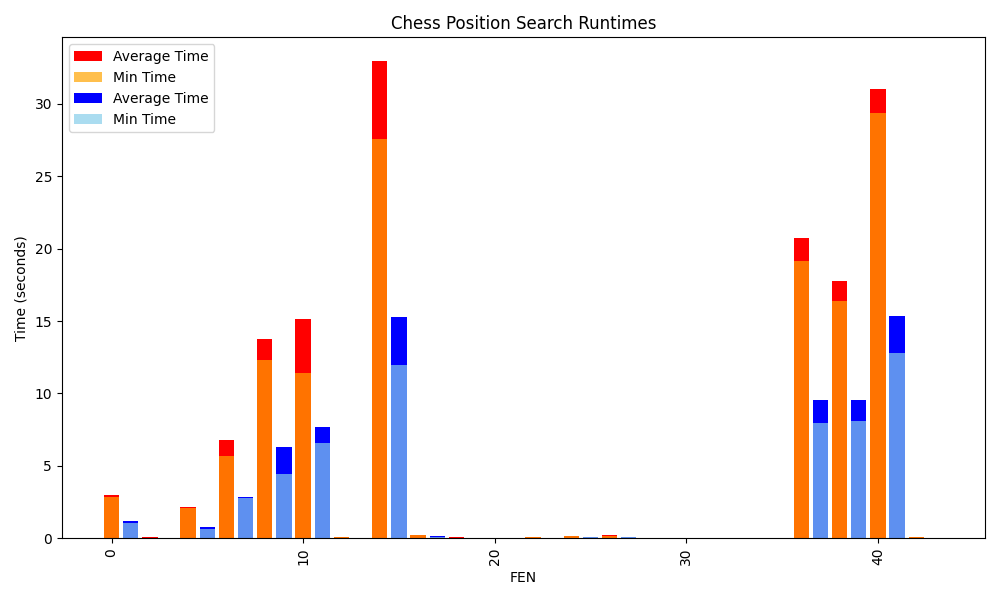
\includegraphics[width=1\linewidth]{recompute-eval-graph.png}
    \caption{The red bars represent the program where the board evaluation was recomputed each time during a depth search. The blue bars are when we cache and update the board evaluation}
    \label{fig:eval-speedup}
\end{figure}

\subsection{Parallelism}
The simplest way to parallelize the move search algorithm is at the top level. Given a board state, we can get all of the moves in that state; then, in parallel, we can use the minimax algorithm to evaluate those results and find the best position for that player.
However, this might not be the most optimal solution, as Figure~\ref{fig:cpu-trace} shows.
This figure shows the CPU utilization over a run of iterative deepening looking for the best move.
The dips in CPU usage are when...
